\documentclass[a4paper,12pt]{report}

\usepackage{alltt, fancyvrb, url}
\usepackage{graphicx}
\usepackage[utf8]{inputenc}
\usepackage{float}
\usepackage{hyperref}
\usepackage[italian]{babel}
\usepackage[italian]{cleveref}

%package

\title{saudio-sim Report}

\author{Alessandro Sciarrillo, Niccolò Mussoni, Alex Presepi, Simone Lugaresi}

\begin{document}

\maketitle

\tableofcontents
\chapter{Analisi}
Il software ha l'obiettivo di permettere all'utente di sperimentare un ascolto realistico in un ambiente dinamico.
%
Per ascolto realistico si intende l'esperienza uditiva che si può sperimentare tramite un ascolto con cuffia che trasmette all'utente effetto di spazialità.
%
Invece con ambiente dinamico ci si riferisce ad un sistema di cui si possono spostare i componenti.

\section{Requisiti funzionali}
\begin{itemize}
	\item  Permettere all'utente di ascoltare tramite le proprie cuffie una riproduzione realistica in relazione alla posizione all'interno di un ambiente personalizzabile.
	\item Garantire all'utente la possibilità di spostare l'ascoltatore e le sorgenti sonore.
		Un ascoltatote ha una posizione all'interno di un ambiente ed è colui nel quale l'utente si impersona.
		Le sorgenti sonore rappresentano i dispositivi da cui il suono viene riprodotto. 
\end{itemize}

\section{Requisiti non funzionali}
\begin{itemize}
	\item L'importazione dovrà supportare anche tracce stereo (2 canali) oltre a quelle mono (1 canale).
\end{itemize}

\section{Analisi e modello del dominio}
desc
%
\begin{figure}[H]
\centering{}
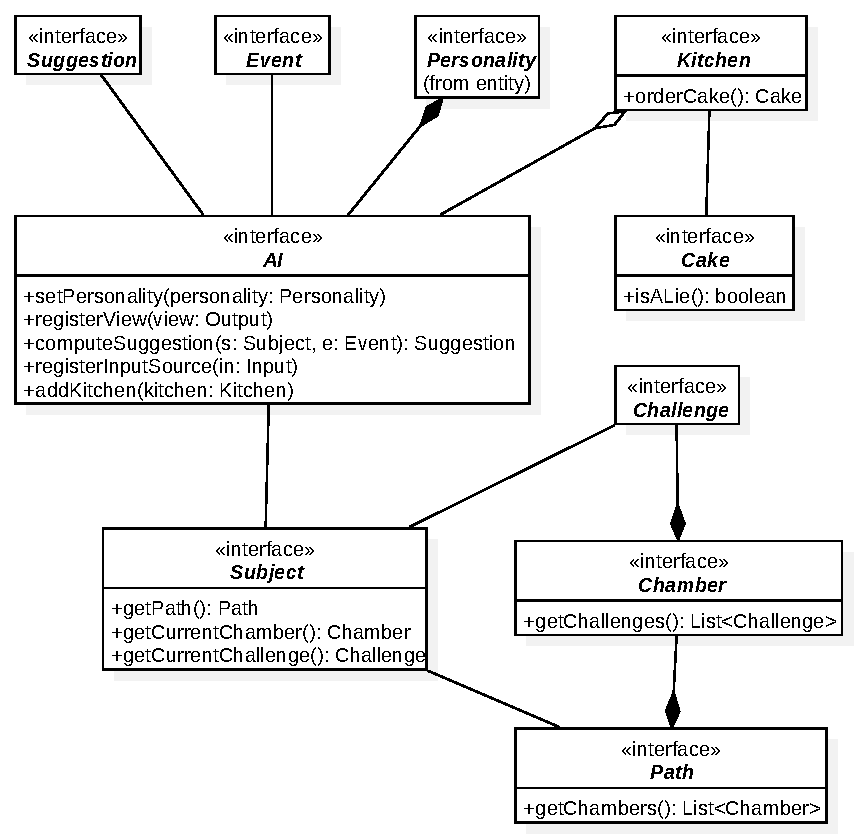
\includegraphics{img/analysis.pdf}
\caption{Schema UML dell'analisi del problema, con rappresentate le entità principali ed i rapporti fra loro}
\label{img:analysis}
\end{figure}


\chapter{Design}

\tableofcontents

\end{document}
